\appendix

\section{Dataset Documentation and Intended Use}
All datasets presented by \name are intended for academic use and their corresponding licenses are listed in Appendix~\ref{app:license}. 
For the ease of access, we provide the following links to the \name benchmark suits and datasets.

\textit{$\bullet$} Dataset and project documentations can be found at: \url{https://tgb.complexdatalab.com/}.

\textit{$\bullet$} \name \texttt{Python} package is available via \texttt{pypi} at: \url{https://pypi.org/project/py-tgb/}.

\textit{$\bullet$} Tutorials and API references can be found at: \url{https://docs.tgb.complexdatalab.com/}.

\textbf{Maintenance Plan.} To provide a robust, realistic, and reproducible benchmark for temporal graphs, we plan to continue developing and maintaining \name based on community feedback and involvement. 
We will maintain and improve the \href{https://shenyanghuang.github.io/TGB/}{TGB} and \href{https://github.com/fpour/TGB_Baselines}{TGB-Baselines} github repository, while the \name datasets are maintained via \href{https://alliancecan.ca/en}{Digital Research Alliance of Canada}~(funded by the Government of Canada). 


\section{Dataset Licenses and Download Links} \label{app:license}

In this section, we present dataset licenses and the download link (embedded in dataset name). 
The datasets are maintained via Digital Reseach Alliance of Canada funded by the Government of Canada.
As authors, we confirm the data licenses as indicated below and that we bear all responsibility in case of violation of rights.

\begin{itemize}[leftmargin=*]
    \item \textbf{\href{https://object-arbutus.cloud.computecanada.ca/tgb/tgbl-wiki-v2.zip}{\wikipedia}:} \underline{MIT license}. The original dataset can be found \href{http://snap.stanford.edu/jodie/#datasets}{here}~\cite{kumar2019predicting}.
    
    \item \textbf{\href{https://object-arbutus.cloud.computecanada.ca/tgb/tgbl-review-v2.zip}{\review}:} \underline{Amazon license}. By accessing the Amazon Customer Reviews Library (a.k.a. \textit{Reviews Library}), one agrees that the Reviews Library is an Amazon Service subject to the \textit{Amazon.com}~\href{https://www.amazon.com/gp/help/customer/display.html/ref=footer_cou?ie=UTF8&nodeId=508088}{Conditions of Use} and one agrees to be bound by them, with the following additional conditions. In addition to the license rights granted under the Conditions of Use, Amazon or its content providers grant the user a limited, non-exclusive, non-transferable, non-sublicensable, revocable license to access and use the Reviews Library for purposes of academic research. One may not resell, republish, or make any commercial use of the Reviews Library or its contents, including use of the Reviews Library for commercial research, such as research related to a funding or consultancy contract, internship, or other relationship in which the results are provided for a fee or delivered to a for-profit organization. One may not (a) link or associate content in the Reviews Library with any personal information (including Amazon customer accounts) or (b) attempt to determine the identity of the author of any content in the Reviews Library. If one violates any of the foregoing conditions, their license to access and use the Reviews Library will automatically terminate without prejudice to any of the other rights or remedies Amazon may have. The original dataset can be found \href{https://nijianmo.github.io/amazon/index.html}{here}~\cite{ni2019justifying}.  
    
    \item \textbf{\href{https://object-arbutus.cloud.computecanada.ca/tgb/tgbl-coin.zip}{\coin}:} \underline{CC BY-NC license} (Attribution-NonCommercial). The original dataset can be found~\href{https://www.chartalist.org/eth/StablecoinAnalysis.html}{here}~\cite{chartalistNeurips2022}.
    
    \item \textbf{\href{https://object-arbutus.cloud.computecanada.ca/tgb/tgbl-comment.zip}{\reddit}:} \underline{CC BY-NC license} (Attribution-NonCommercial).  The original dataset can be found~\href{https://surfdrive.surf.nl/files/index.php/s/M09RDerAMZrQy8q}{here}~\cite{nadiri2022large}.
    
    \item \textbf{\href{https://object-arbutus.cloud.computecanada.ca/tgb/tgbl-flight.zip}{\sky}:} a non-commercial, limited, non-exclusive, non-transferable, non-assignable, and terminable license to copy, modify, and use the data in accordance with this agreement solely for the purpose of non-profit research, non-profit education, commercial internal testing and evaluation of the data, or for government purposes. No license is granted for any other purpose and there are no implied licenses in this agreement. For more details, please consult the \href{https://zenodo.org/record/7323875}{original dataset license}. The original dataset can be found \href{https://zenodo.org/record/7323875#.ZEmhTnZKguU}{here}~\cite{strohmeier2021crowdsourced}.
    
    \item \textbf{\href{https://object-arbutus.cloud.computecanada.ca/tgb/tgbn-trade.zip}{\trade}:} \underline{MIT license}. The original dataset can be found \href{https://www.fao.org/faostat/en/#data/TM}{here}~\cite{macdonald2015rethinking}.
    
    \item \textbf{\href{https://object-arbutus.cloud.computecanada.ca/tgb/tgbn-genre.zip}{\fm}:} \underline{MIT license}. The original \textit{LastFM-song-listens} dataset~\cite{kumar2019predicting,hidasi2012fast} and the \textit{million-song} dataset~\cite{bertin2011million} is available \href{http://snap.stanford.edu/jodie/#datasets}{here} and \href{http://millionsongdataset.com/}{here}, respectively. 
    
    \item \textbf{\href{https://object-arbutus.cloud.computecanada.ca/tgb/tgbn-reddit.zip}{\subreddit}:} \underline{CC BY-NC license} (Attribution-NonCommercial). The original dataset can be found~\href{https://surfdrive.surf.nl/files/index.php/s/M09RDerAMZrQy8q}{here}~\cite{nadiri2022large}. 

    \item \changed{\textbf{\href{https://object-arbutus.cloud.computecanada.ca/tgb/tgbn-token.zip}{\token}:} \underline{CC BY-NC license} (Attribution-NonCommercial). The original dataset can be found~\href{https://chartalist.org/eth/TaskMultilayer.html}{here}~\cite{chartalistNeurips2022}}.
    
\end{itemize}



\section{Evaluation Settings in TG} \label{app:eval}

Based on how the test set information is used during the evaluation of temporal graph learning models, the existing approaches can be grouped into the following three categories.
We emphasize that methods from different categories should be evaluated distinctly to avoid unfair comparison. 
Following the practice of the previous works and for the sake of clarity, we comply with \emph{streaming setting}.
Particularly, we consider a fixed split point in time, i.e. \textit{$t_{split}$}, where the information before and after this point constitute the training and test data, respectively.

\paragraph{Streaming Setting.} In this setting, information from the test set is only employed for updating the \textit{memory} module in temporal graph learning methods (e.g., TGN~\cite{rossi2020temporal}). 
However, no back-propagation or model update is possible based on the test set information. 
We consider this setting as \textit{streaming}, since it helps in fast inference by incorporating the recent information (even from the test set), while observign the fact that retraining the model with the test data is too expensive.
 
\paragraph{Deployed Setting.} In this setting, the test set information is not available for any modification to the model. 
This setting closely follows the standard machine learning setting with distinct training dataset and test dataset. We refer to this setting as \textit{deployed} to denote that after deploying the a model, it is only used for inference and no updates to any part of the model is allowed. 

\paragraph{Live-Update Setting.} In this setting, information from any point in the past (including the test set information) can be used to re-train, fine-tune, or update the model. 
The goal of this setting is to achieve the best prediction for each timestamp \textit{$t+1$} given the historical information at all previous timestamps in~\textit{$[0,...,t]$}. 
We consider this setting as \textit{live-update} because the model weights can be updated lively through the incoming data.
Note that this setting is similar to the rolling setting exercised in ROLAND framework~\cite{you2022roland}.

\section{Temporal Graph Learning Models} \label{app:methods}

Recently, there is an increasing interest in developing graph representation learning models for networks that evolve over times. 
Evolving graphs can be investigated at different time granularity.
\changed{
Kazemi \emph{et al.}~\cite{kazemi2020representation} categorize temporal graphs into Discrete Time Dynamic Graphs~(DTDGs) and Continous Time Dynamic Graphs~(CTDGs). 
DTDGs consist of an ordered set of static graph snapshots while CTDGs compose of timestamped edge streams where edges are denoted by triplets of source, destination, and timestamp.
% as well as node events. 
DTDG models specialize in sequences of graph snapshots capturing the dynamics of a temporal graph where these snapshots are sampled at regular time intervals~\cite{you2022roland, gao2022equivalence,pareja2020evolvegcn,hajiramezanali2019variational,yang2021discrete}. 
In contrast, CTDG methods often aggregating the features from temporal neighborhood (connected nodes with close time proximity) and constantly adjusting the encoding as edge stream continues~\cite{rossi2020temporal,wanginductive,luoneighborhood}. 
In this work, we primarily focus on CTDGs, driven by several compelling reasons.
First, CTDG models which employs the precise temporal information offered by CTDGs, can be effectively utilized for DTDGs.
On the contrary, adapting DTDG models for drawing inferences from CTDGs is a non-trivial task.
Second, it has been shown that DTDGs are convertible to CTDGs \cite{souza2022provably}, while the conversion in the opposite direction results in loss of information.
Next, we introduce the methods used in our evaluation for the dynamic link property prediction and dynamic node property prediction task.
}

\textbf{Models Used for Evaluation of Dynamic Link Property Prediction Task.}
\begin{itemize}[leftmargin=*]
    \item \emph{DyRep}~\cite{trivedi2019dyrep} is a temporal point process-based model that propagates interaction messages via Recurrent Neural Networks~(RNNs) to update the node representations. It employs a temporal attention mechanism to model the weights of a given node's neighbors. 
    
    \item \emph{TGN}~\cite{rossi2020temporal} is a general framework for learning on continuous time dynamic graphs. It has the following components: memory module, message function, message aggregator, memory updater, and embedding module. TGN updates the node memories at test time with newly observed edges. 
    
    \item \emph{GraphMixer}~\cite{congwe} is a simple model for dynamic link prediction consisting of three main modules: a node-encoder to summarize the node information, a link-encoder to summarize the temporal link information, and a link predictor module. These modules that only employ based on multi-layer perceptrons~(MLPs), making GraphMixer a simple model without the use of a GNN architecture.
    
    \item \emph{TCL}~\cite{wang2021tcl} employs a transfomer module to generate temporal neighborhood representations for nodes involved in an interaction. 
    It then models the inter-dependencies with a co-attentional transfomer at a semantic level. Specifically, TCL utilizes two separate encoders to extract representations from temporal neighborhoods surrounding the two nodes of an edge.
    
    \item \emph{CAWN}~\cite{wanginductive} predicts dynamic links based on extracting temporal random walks and retrieves temporal network motifs to represent network dynamics. It utilizes a neural network model to encode Causal Anonymous Walks~(CAWs) to support online training and inference.
    Particularly, it starts by relabeling nodes with encoded temporal anonymous walks starting at the nodes involved in an interaction.
    Then, the temporal walks themselves are further encoded using the generated node labels and encodings of the elapsed times.
    Finally, the existence of a link is predicted based on aggregating the walks encoding through a pooling module.

    \item \changed{\emph{TGAT}~\cite{xu2020inductive} captures both temporal and structural characteristics of dynamic graphs using a self-attention mechanism. 
    At a specific timestamp \textit{$t$}, TGAT first concatenates the raw features of a node with a trainable encoding of time \textit{$t$}.
    Upon the observation of an interaction among a pair of nodes, TGAT utilizes the self-attention mechanism to apply message passing to the time augmented node features and generates the latest node representations.}

    \item \changed{\emph{NAT}~\cite{luoneighborhood} adopts a novel dictionary-type neighborhood representation for nodes. Such representation records a downsampled set of node neighbors as keys and constructs features for joint neighborhood of multiple nodes. A dedicated data structure called N-cache supports GPU acceleration for the dictionary representations.}
    
    \item $\text{\emph{EdgeBank}}_{\infty}$~\cite{poursafaeitowards} is a simple heuristic storing all observed edges in a memory (implemented as a hashtable). 
    At inference time, if the queried node pair is in the memory then $\text{EdgeBank}_{\infty}$ predicts true, otherwise $\text{EdgeBank}_{\infty}$ predicts false.
    
    \item $\text{\emph{EdgeBank}}_{\text{tw}}$~\cite{poursafaeitowards} is another variation of EdgeBank which only memorizes edges from a fixed duration in the recent past. Therefore, it has a strong recency bias.  
\end{itemize}

\textbf{Models Used for Evaluation of Dynamic Node Property Prediction Task.}
\begin{itemize}[leftmargin=*]
    \item \emph{TGN}~\cite{rossi2020temporal} is discussed above. We utilize the TGN embedding of a node from the memory at the query time $t$ to predict the node labels.  

    \item \emph{DyRep}~\cite{trivedi2019dyrep} same as discussed above. We use the node embedding to predict the node labels. 
    
    \item \emph{Persistant Forecast}~\cite{salcedo2022persistence} is a simple yet powerful baseline for time series forecasting and complex systems. Here, we extend the core idea by simply outputting the recently observed node label for the current time $t$. 
    
    \item \emph{Moving Average}~\cite{panch2018artificial} considers the average of the node labels observed in the previous $k$ steps (we set $k=7$). 
\end{itemize}


\section{Computing Resources}
\label{sec:comp_resources}

\textbf{Dynamic link property prediction.} For this task, we ran all experiments on either \href{https://docs.alliancecan.ca/wiki/Narval/en}{Narval} or \href{https://docs.alliancecan.ca/wiki/Béluga/en}{Béluga} cluster of \href{https://www.alliancecan.ca/en}{Digital Research Alliance of Canada}.
For the experiments on Narval cluster, we ran each experiment on a Nvidia A100 (40G memory) GPU with 4 CPU nodes (from either of the AMD Rome 7532 @ 2.40 GHz 256M cache L3, AMD Rome 7502 @ 2.50 GHz 128M cache L3, or AMD Milan 7413 @ 2.65 GHz 128M cache L3 available type) each with 100G memory.
For the experiments on Béluga, we ran each experiment on a NVidia V100SXM2 (16G memory) GPU with 4 CPU nodes (from either of the Intel Gold 6148 Skylake @ 2.4 GHz, Intel Gold 6148 Skylake @ 2.4 GHz, Intel Gold 6148 Skylake @ 2.4 GHz, or Intel Gold 6148 Skylake @ 2.4 GHz) each with 100G memory.
A five-day time limit is considered for each experiment.
We repeated each experiments five times and reported the average and standard deviation of different runs.
It is noteworthy that except for the TGN~\cite{rossi2020temporal} and DyRep~\cite{trivedi2019dyrep} models that we ported them into the PyTorch Geometric environment, the other models (evaluated by their original source code or by using the \href{https://github.com/yule-BUAA/DyGLib}{DyGLib} repository) throw an \textit{out of memory} error for the medium and large datasets on both Narval and Béluga clusters.

\textbf{Dynamic Node Property Prediction} For this task, we ran experiments with 4 standard CPU and either RTX8000, V100, A100 or A6000 GPUs. \changed{The longest experiment takes around 2 days on the \reddit and \token dataset.}

\section{GPU Usage Comparison} \label{app:gpu}

\begin{figure}[t]
\centering
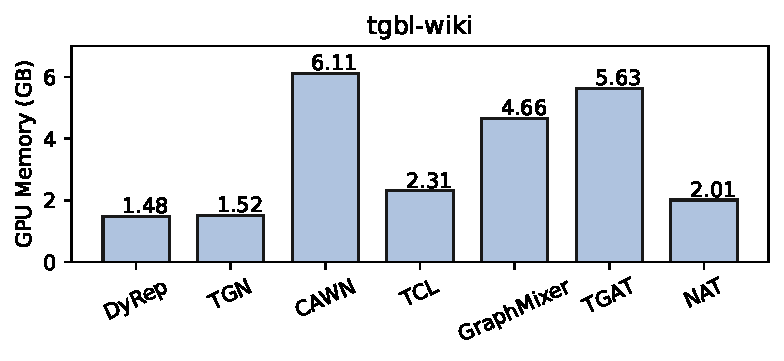
\includegraphics[width=0.7\linewidth]{figs/time/tgbl-wiki_gpu.pdf}
\caption{\changed{GPU Memory Usage for \textcolor[HTML]{e7298a}{\wikipedia} dataset.}}
\label{Fig:gpu}
\end{figure}

\changed{ In Figure~\ref{Fig:gpu}, we report the average GPU usage of TG methods on the \wikipedia dataset across 5 trials. Note that EdgeBank is a heuristic and only requires CPU thus no GPU usage is reported. Some methods such as GraphMixer has significantly higher GPU usage when compared to others while most methods have similar GPU usage. 
}



\section{Additional Dataset Statistics} \label{app:stats}


\setlength\tabcolsep{2.2pt}
\begin{table*}[t] %\vspace{-12pt}
\caption{\changed{Additional dataset properties. Dataset names are colored based on their scale as \textcolor[HTML]{e7298a}{small}, \textcolor{blue}{medium}, and \textcolor[HTML]{1b9e77}{large}. \textit{$\star$}: denotes the average number of edges per timestamp.}} %\vspace{-5pt}
\label{tab:stats-extra}
  \resizebox{\textwidth}{!}{%
  
  \begin{tabu}{l l | c c | c c | c c | l | l }
  \toprule
  % & Dataset & Val. nn. ratio &  Test nn. ratio  & \# Val new nodes & \# Test new nodes \\
  \rowfont{\color{revised}}
  & \multirow{2}{*}{Dataset} & \multicolumn{2}{c |}{ inductive node ratio}  &  \multicolumn{2}{c |}{ \# inductive nodes} & \multicolumn{2}{c|}{total \# nodes} & \multirow{2}{*}{\textit{$|\overline{E_t}|^\star$}} & \multirow{2}{*}{Reoccurrence} \\
  \rowfont{\color{revised}}
  &         & Val. & Test  & Val. & Test & Val. & Test &   &  \\

  %& Time Granularity
  \midrule
  \rowfont{\color{revised}}
  \multirow{5}{*}{\rotatebox[origin=c]{90}{\textbf{Link}}} & \textcolor[HTML]{e7298a}{\wikipedia} & 0.257 & 0.308 & 836 & 1,099 & 3,256 & 3,564 & 1.031 & 0.015\\
  \rowfont{\color{revised}}
   & \textcolor[HTML]{e7298a}{\review}                          & 0.024 & 0.027 & 5,728 & 6,336 & 242,820 & 234,641 & 709.911 & 0.0002 \\
   \rowfont{\color{revised}}
   & \textcolor{blue}{\coin}                                    & 0.112 & 0.174 & 37,689 & 336,161 & 55,781 & 321,008 & 17.604 & 0.025 \\
   \rowfont{\color{revised}}
   & \textcolor[HTML]{1b9e77}{\reddit}                          & 0.474 & 0.562 & 137,424 & 177,558 & 289,713 & 315,662 & 1.430 & 0.006\\
   \rowfont{\color{revised}}
   & \textcolor[HTML]{1b9e77}{\sky}                            & 0.031 & 0.045 & 474 & 689  & 15,170 & 15,347 & 48497.884 & 0.009 \\
  
  \midrule
  \rowfont{\color{revised}}
  \multirow{3}{*}{\rotatebox[origin=c]{90}{\textbf{Node}}} & \textcolor[HTML]{e7298a}{\trade}  & 0.009 & 0.009 & 2 & 2 & 216 & 228 & 15104.677 & 0.052\\
  \rowfont{\color{revised}}
  & \textcolor{blue}{\fm}                                                                       & 0.056 & 0.097 & 70 & 129 & 1,260 & 1,328 & 4.265 & 0.003\\
  \rowfont{\color{revised}}
  & \textcolor[HTML]{1b9e77}{\subreddit}                                                        & 0.031 & 0.035 & 349 & 390 & 11,191 & 11,099  & 1.241 & 0.009\\
  \rowfont{\color{revised}}
   & \textcolor[HTML]{1b9e77}{\token}                                                           & 0.086 & 0.076 & 4,013 & 3,178 & 46,541 & 42,023  & 35.81 & 0.002\\              
  % \bottomrule
  \bottomrule
  \end{tabu}
  }
%\vspace{-10pt}
\end{table*}


In addition to the main dataset statistics presented in Table~\ref{tab:stats-summarized}, it is insightful to examine some other dataset characteristics as indicated in Table~\ref{tab:stats-extra}.
The \emph{reoccurence index} (i.e., \textit{$\frac{|E_\text{train} \cap {E_\text{test}}|} {|E_\text{train}|}$}) denotes the ratio of training edges that reoccur during the test phase as well.
If the edges appearance follows a consistent pattern, a high \emph{reoccurrence index} can be correlated with the high performance of a memorization-based approach such as EdgeBank~\cite{poursafaeitowards}.
The average number of edges per timestamps provides information about the evolution of the datasets, and the ratio of the new nodes in validation or test set provides insights about the portion of unseen nodes introduced during inference.
It should be noted that although we mainly focus on \textit{transductive} dynamic link property prediction task in our evaluation, the ratio of new nodes in validation or test set (fourth and fifth column in Table~\ref{tab:stats-extra}) show that there are indeed new nodes during the validation and test phase.
Correctly predicting the properties of edges for the new nodes might be more challenging for the models, since no historical information about these nodes are available. Lastly, we observe that \name datasets are also diverse in all of the above properties.

\section{Number of Negative Samples} \label{app:ns}
\changed{
To study the effect of the number of negative samples, here we report the results for the \textcolor[HTML]{e7298a}{small} link property prediction datasets in TGB with \emph{20} negative samples in Table~\ref{tab:wiki-20} and~\ref{tab:review-20} for \wikipedia and \review respectively across five trials.
When contrasting these findings with those presented in Table~\ref{tab:wiki} and~\ref{tab:review}, which involve a higher quantity of negative samples, the insights outlined in Section~\ref{sec:exp} are reaffirmed.
For example, there is a significant drop in performance for the top performing method, i.e. CAWN, from \wikipedia to \review. 
In addition, Edgebank performance has a significant drop when the surprise index is high on (which is the case in \review). 
However, we can also clearly see that with lower number of negatives (particularly on \wikipedia), the MRR scores are significantly higher for most methods. Therefore, if computationally feasible, it is best to use more negative samples. 
In our case, more negative samples are used for \textcolor[HTML]{e7298a}{small} TGB datasets. 
}


\begin{table*}[t]
\caption{ \changed{Results for \emph{dynamic link property prediction} on \textcolor[HTML]{e7298a}{small} datasets with \emph{20} negative samples.}}
\begin{subtable}[t]{0.5\textwidth}
\resizebox{0.9\textwidth}{!}{
\begin{tabular}{ l | l l}
  \toprule
  \multirow{2}{*}{Method}    &   \multicolumn{2}{c}{\textbf{\textbf{MRR}}} \\
                           & Validation     & Test  \\
   \midrule
    DyRep~\cite{trivedi2019dyrep}              & 0.411\scriptsize{$\pm$0.015}   & 0.366\scriptsize{$\pm$0.014} \\
    TGN~\cite{rossi2020temporal}               & \underline{0.737}\scriptsize{$\pm$0.004}  & \underline{0.721}\scriptsize{$\pm$0.004}  \\
    CAWN~\cite{wanginductive}                  & \textbf{0.794}\scriptsize{$\pm$0.014}   & \textbf{0.791}\scriptsize{$\pm$ 0.015} \\
    % TGAT~\cite{xu2020inductive}                  & 0.690\scriptsize{$\pm$0.011} &  0.668\scriptsize{$\pm$0.0114}\\
    TCL~\cite{wang2021tcl}                      & 0.734\scriptsize{$\pm$0.007}   & 0.712\scriptsize{$\pm$0.007}  \\
    GraphMixer~\cite{congwe}                     & 0.707\scriptsize{$\pm$0.014}   & 0.701\scriptsize{$\pm$0.014}  \\
    % \midrule
    $\text{EdgeBank}_{\text{tw}}$~\cite{poursafaeitowards}   & 0.641  & 0.641 \\
    $\text{EdgeBank}_{\infty}$~\cite{poursafaeitowards}      & 0.551 & 0.538  \\
    \bottomrule
\end{tabular}
}
\caption{\textcolor[HTML]{e7298a}{\wikipedia} dataset with \emph{surprise index}: $0.108$. \\ (with \emph{20} negative edges per positive edge).}
\label{tab:wiki-20}
\end{subtable}%
\begin{subtable}[t]{0.5\textwidth}
\resizebox{0.9\textwidth}{!}{
\begin{tabular}{ l | l l}
  \toprule
  \multirow{2}{*}{Method}    &   \multicolumn{2}{c}{\textbf{\textbf{MRR}}} \\
                            & Validation     & Test  \\
   \midrule
    DyRep~\cite{trivedi2019dyrep}             & 0.356\scriptsize{$\pm$0.016}  & 0.367\scriptsize{$\pm$0.013}  \\
    TGN~\cite{rossi2020temporal}                & \textbf{0.465}\scriptsize{$\pm$0.010}  & \textbf{0.532}\scriptsize{$\pm$0.020}\\
    CAWN\cite{wanginductive}               & 0.201\scriptsize{$\pm$0.002}   & 0.194\scriptsize{$\pm$0.004} \\
    % TGAT~\cite{xu2020inductive}               & xxx \scriptsize{xxx}   & xxx \scriptsize{xxx}\\
    TCL~\cite{wang2021tcl}                & 0.194\scriptsize{$\pm$0.012} & 0.200 \scriptsize{$\pm$0.010} \\
    GraphMixer~\cite{congwe}         & \underline{0.411}\scriptsize{$\pm$0.025}  & \underline{0.514}\scriptsize{$\pm$0.020} \\
    % \midrule
    $\text{EdgeBank}_{\text{tw}}$~\cite{poursafaeitowards}   & 0.0894 & 0.0836   \\
    $\text{EdgeBank}_{\infty}$~\cite{poursafaeitowards}      & 0.0786      & 0.0795    \\
    \bottomrule
\end{tabular}
}
\caption{\textcolor[HTML]{e7298a}{\review} dataset with \emph{surprise index}: $0.987$. \\ (with \emph{20} negatives edges per positive edge).}
\label{tab:review-20}
\end{subtable}%
\vspace{-10pt}
\end{table*}


\section{Transductive and Inductive Comparison}

\begin{table*}[t]
\caption{\changed{Transductive vs. Inductive Setting on \textcolor[HTML]{e7298a}{\wikipedia} Dataset.}}
\centering
\resizebox{0.7\textwidth}{!}{
\begin{tabu}{ l | l l | l l}
  \toprule
  \rowfont{\color{revised}}
  \multirow{2}{*}{Method}    & \multicolumn{2}{c|}{\textbf{\textbf{Val. MRR}}} &   \multicolumn{2}{c}{\textbf{\textbf{Test MRR}}} \\
  \rowfont{\color{revised}}
                           &  Transductive    & Inductive &  Transductive    & Inductive  \\
   \midrule
   \rowfont{\color{revised}}
    DyRep~\cite{trivedi2019dyrep}   & 0.058\scriptsize{$\pm$0.013} & 0.049\scriptsize{$\pm$0.021}           & 0.040\scriptsize{$\pm$0.017}   & 0.053\scriptsize{$\pm$0.021}  \\
    \rowfont{\color{revised}}
    TGN~\cite{rossi2020temporal}   & 0.395\scriptsize{$\pm$0.028} &  0.231\scriptsize{$\pm$0.028}   & 0.325\scriptsize{$\pm$0.055}  & 0.268\scriptsize{$\pm$0.043}  \\
    \rowfont{\color{revised}}
    TCL~\cite{wang2021tcl}        & 0.187\scriptsize{$\pm$0.012}   & 0.212\scriptsize{$\pm$0.016}  & 
    0.194\scriptsize{$\pm$0.014}  & 0.182\scriptsize{$\pm$0.009}  \\
    \rowfont{\color{revised}}
    GraphMixer~\cite{congwe}      & 0.113\scriptsize{$\pm$0.005}   & 0.130\scriptsize{$\pm$0.004}  &
    0.122\scriptsize{$\pm$0.005}  & 0.107\scriptsize{$\pm$0.005}   \\
    \rowfont{\color{revised}}
    NAT~\cite{luoneighborhood}    &  \textbf{0.784}\scriptsize{$\pm$0.012} &  \textbf{0.745}\scriptsize{$\pm$0.002} &
    \textbf{0.763}\scriptsize{$\pm$0.011}  & \textbf{0.717}\scriptsize{$\pm$0.005} \\    
    \rowfont{\color{revised}}
    CAWN~\cite{wanginductive}                  & \underline{0.749}\scriptsize{$\pm$0.009}   & \underline{0.742}\scriptsize{$\pm$ 0.004} 
    & \underline{0.720}\scriptsize{$\pm$0.010}   & \underline{0.709}\scriptsize{$\pm$ 0.005}\\
    \rowfont{\color{revised}}
    TGAT~\cite{xu2020inductive}                 &   0.147\scriptsize{$\pm$0.009} & 0.150\scriptsize{$\pm$0.020}
    & 0.155\scriptsize{$\pm$0.007}  & 0.152\scriptsize{$\pm$ 0.016}\\
    % TCL~\cite{wang2021tcl}                      & xxx\scriptsize{$\pm$0.016}   & xxx\scriptsize{$\pm$0.025}  \\
    % GraphMixer~\cite{congwe}                     & xxx\scriptsize{$\pm$0.003}   & xxx\scriptsize{$\pm$0.002}  \\
    % NAT~\cite{luoneighborhood}                   &  \textbf{0.773}\scriptsize{$\pm$0.011} &  \textbf{0.749}\scriptsize{$\pm$0.010}    \\
    % \midrule
    \rowfont{\color{revised}}
    $\text{EdgeBank}_{\text{tw}}$~\cite{poursafaeitowards} & 0.605 & 0.566  & 0.575  & 0.551 \\
    \rowfont{\color{revised}}
    $\text{EdgeBank}_{\infty}$~\cite{poursafaeitowards}  & 0.520 & 0.566 & 0.481 & 0.562  \\
    \bottomrule
\end{tabu}
}
\end{table*}

\changed{
In this section, we compare method performance following the commonly used transductive and inductive setting as seen in prior literature~\cite{xu2020inductive, wanginductive} across five trials. We define inductive nodes as nodes that are unseen in the training set and transduction nodes as nodes that are observed in the training set. The transductive MRR is computed from all edges which has a transdustive source node and inductive MRR is computed from all edges that has an inductive source node respectively. We observe that for a method to achieve strong performance on \wikipedia such as NAT, it should perform well in both transductive and inductive reasoning. }



\section{Additional Computational Time Comparison} \label{app:time}

\begin{figure}[t]
\centering
\begin{subfigure}{.3\textwidth}
  \centering
  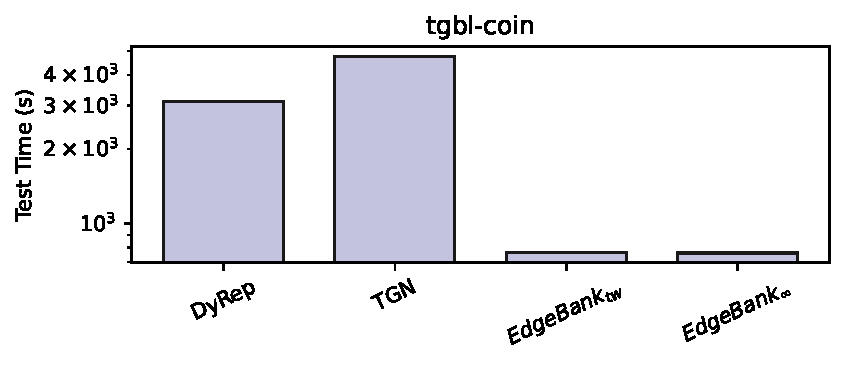
\includegraphics[width=\linewidth]{figs/time/tgbl-coin_test_time.pdf}
  \caption{\textcolor{blue}{\coin} dataset.}
  \label{Fig:coin_test}
\end{subfigure}%
\begin{subfigure}{.3\textwidth}
  \centering
  %
\includegraphics[width=.4\linewidth]{image1}
  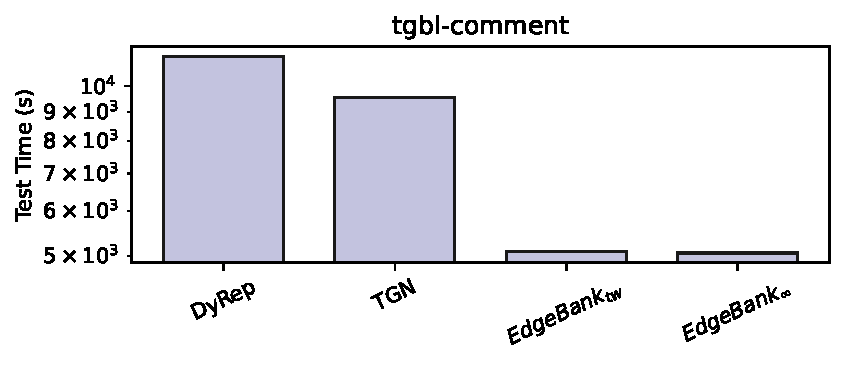
\includegraphics[width=\linewidth]{figs/time/tgbl-comment_test_time.pdf}
  \caption{\textcolor[HTML]{1b9e77}{\reddit} dataset.} 
  \label{Fig:comment_test}
\end{subfigure}
\begin{subfigure}{.3\textwidth}
  \centering
  %
\includegraphics[width=.4\linewidth]{image1}
  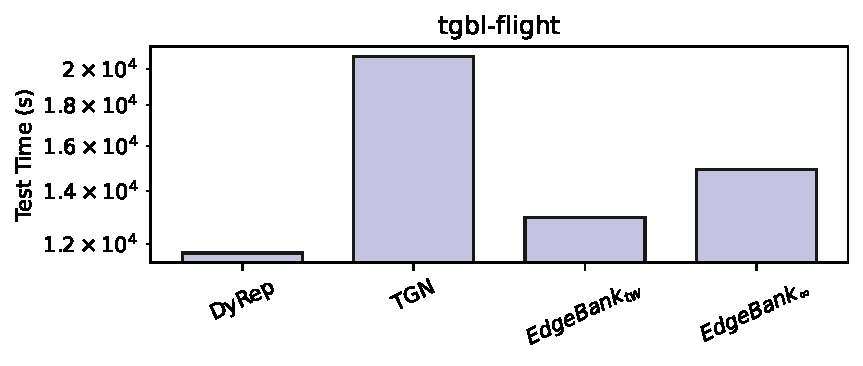
\includegraphics[width=\linewidth]{figs/time/tgbl-flight_test_time.pdf}
  \caption{\textcolor[HTML]{1b9e77}{\sky} dataset.} 
  \label{Fig:flight_test}
\end{subfigure}
\caption{\changed{Inference time comparison of TG methods.}}
\end{figure}

\changed{Here, we report additional results for computational time comparison on \coin, \sky and \reddit datasets. Figure~\ref{Fig:coin_test},~\ref{Fig:comment_test} and~\ref{Fig:flight_test} reports the test time for TG methods on \coin, \sky and \reddit respectively. On both \coin and \reddit, Edgebank is one order of magnitude faster than TGN and DyRep. On the \sky, due to the large number of edges, DyRep is the fastest.}




% % ! moved to main paper
% \section{Node Property Prediction Updated}
% \changed{Here is the updated results for node property prediction with improvements suggested in~\cite{yu2023empirical}.}


% \begin{table*}[t]
% \caption{\changed{\emph{Dynamic node property prediction} results across 5 trials (updated results).}} 
% \label{tab:nodepred}
% \centering
% \resizebox{\textwidth}{!}{
%   \begin{tabular}{l | l l | l l | l l | l l}
%   \toprule
%   \multirow{3}{*}{Method} &  \multicolumn{2}{c|}{\textcolor[HTML]{e7298a}{\trade}}  & \multicolumn{2}{c|}{\textcolor{blue}{\fm}} & \multicolumn{2}{c|}{\textcolor[HTML]{1b9e77}{\subreddit}} & \multicolumn{2}{c}{\textcolor[HTML]{1b9e77}{\token}} \\
%    & \multicolumn{2}{c|}{\textbf{NDCG@10}}       & \multicolumn{2}{c|}{\textbf{NDCG@10}} & \multicolumn{2}{c}{\textbf{NDCG@10}} & \multicolumn{2}{c}{\textbf{NDCG@10}} \\
%        & Validation  & Test                & Validation    & Test             & Validation      & Test & Validation      & Test \\
%        \midrule
%     DyRep~\cite{trivedi2019dyrep}    & 0.394\scriptsize{$\pm$0.001} & 0.374\scriptsize{$\pm$0.001} & 0.357\scriptsize{$\pm$0.001} & 0.351\scriptsize{$\pm$0.001} & 0.344\scriptsize{$\pm$ 0.001} & 0.312\scriptsize{$\pm$ 0.001}
%     & 0.151\scriptsize{$\pm$ 0.006} & 0.141\scriptsize{$\pm$ 0.006}\\

%     TGN~\cite{rossi2020temporal}      & 0.395\scriptsize{$\pm$0.002} & 0.374\scriptsize{$\pm$0.001} & 0.403\scriptsize{$\pm$0.010} & 0.367\scriptsize{$\pm$0.058} & 0.379\scriptsize{$\pm$ 0.004} & 0.315\scriptsize{$\pm$ 0.020}  
%     & 0.189\scriptsize{$\pm$ 0.005} & 0.169\scriptsize{$\pm$ 0.006}\\
%     % \midrule
%     persistence Fore.~\cite{salcedo2022persistence} & \textbf{0.860}  & \textbf{0.855} & 0.350    & 0.357 & 0.380   & 0.369 & 0.403 & 0.430\\
%     Moving Avg.~\cite{panch2018artificial}      & 0.841   & 0.823 & \textbf{0.499} & \textbf{0.509} & \textbf{0.574}    & \textbf{0.559} & \textbf{0.491} & \textbf{0.508}\\
%   \bottomrule
%   \end{tabular}
% }
% \end{table*}



% \setlength\tabcolsep{2.2pt}
% \begin{table*}[t] %\vspace{-12pt}
% \caption{Additional dataset properties. Dataset names are colored based on their scale as \textcolor[HTML]{e7298a}{small}, \textcolor{blue}{medium}, and \textcolor[HTML]{1b9e77}{large}.} %\vspace{-5pt}
% \label{tab:stats-extra}
%   \resizebox{\textwidth}{!}{%
  
%   \begin{tabular}{l l | l l l l}
%   \toprule
%   \toprule
%    & Dataset & Avg. \#edges per ts & Reoccurrence & Val. new-node ratio &  Test new-node ratio  \\
%   %& Time Granularity
%   \midrule
%   \multirow{5}{*}{\rotatebox[origin=c]{90}{\textbf{Link}}} & \textcolor[HTML]{e7298a}{\wikipedia} & 1.031 & 0.015 & 0.257 & 0.257 \\
%    & \textcolor[HTML]{e7298a}{\review}                          & 709.911 & 0.0002 & 0.0024 & 0.008 \\
%    & \textcolor{blue}{\coin}                            & 17.604 & 0.025 & 0.112 & 0.081 \\
%    & \textcolor[HTML]{1b9e77}{\reddit}                          & 1.430 & 0.006 & 0.474 & 0.397 \\
%    & \textcolor[HTML]{1b9e77}{\sky}                            & 48497.884 & 0.009 & 0.031 & 0.021 \\
  
%   \midrule
%   \multirow{3}{*}{\rotatebox[origin=c]{90}{\textbf{Node}}} & \textcolor[HTML]{e7298a}{\trade}     & 15104.677 & 0.052 & 0.009 & 0.000 \\
%   & \textcolor{blue}{\fm}                              & 4.265 & 0.003 & 0.056 & 0.046 \\
%   & \textcolor[HTML]{1b9e77}{\subreddit}                        & 1.241 & 0.009 & 0.031 & 0.004 \\
%   \bottomrule
%   \bottomrule
%   \end{tabular}
%   }
% %\vspace{-10pt}
% \end{table*}




% \section{Additional Task Details} \label{app:task}
% \changed{In this section, we discuss more details about the task and its impact for each of the TGB datasets.}


% \changed{\underline{\textbf{\sky.}} In this dataset, the task is to predict if a flight will exist from a given airport to another in a future date. This is important for predicting future flight disruptions such as cancellation and delays. For example, during the COVID-19 pandemic, many flight routes are cancelled to combat the spread of COVID-19. In addition, the prediction of global flight network is also important for studying and forecasting the spread of disease such as COVID-19 to new regions, as shown in~\cite{ding2021incorporating}.}




% To learn the dynamic representations, \textit{JODIE}~\cite{kumar2019predicting} updates the node representations after each interaction by two decoupled RNNs with time-dependent projection.
% \textit{DyRep}~\cite{trivedi2019dyrep} is temporal point process-based model that propagates interaction messages via RNNs to update the node representations.
% \textit{TGN}~\cite{rossi2020temporal} is a general framework for learning on continuous time dynamic graphs.
% Similar to TGAT~\cite{xu2020inductive}, it employs a temporal graph attention module to capture temporal and structural information.
% TGN also has a RNN-based memory module to store the history of the events in which a node was involved.
% \textit{CAWN}~\cite{wanginductive} predicts dynamic links using casual anonymous walks.
% First, it relabels nodes with encoding temporal anonymous walks starting at the nodes involved in an interaction.
% Then, the temporal walks themselves are encoded using the generated node labels and encodings of the elapsed times.
% Finally, the existence of a link is predicted based on aggregating the walks encoding through a pooling module.
% \textit{TCL}~\cite{wang2021tcl} employs a transfomer module to generate temporal neighborhood representations for nodes involved in an interaction. 
% It then models the inter-dependencies with a co-attentional transfomer at a semantic level.
% \textit{PINT}~\cite{souza2022provably} first categorizes temporal graph network models into two main categories namely message passing- and temporal random walk-based models, and investigates the strength and limitations of each categories.
% Then, it extends the 1-WL (Weisfeiler-Leman) test to temporal graphs.
% Finally, the authors combine injective temporal message passing and relative positional encoding to propose a powerful and more expressive temporal graph learning model.
% \textit{NAT}~\cite{luoneighborhood} stores node-level and link-level representations for each node.
% The authors designed a especial data structure that facilitates fast construction of joint neighborhood structural features.
% The proposed model provides a good model scalability by incorporating dictionary-type neighborhood representations and helps to achieve fast link prediction.
% \textit{GraphMixer}~\cite{congwe} is a straightforward models for dynamic link prediction consisting of three main modules: 
% a node-encoder to summarize the node information, 
% a link-encoder to summarize the temporal link information,
% and a link predictor module.


% Long-term preservation: It must be clear that the dataset will be available for a long time, either by uploading to a data repository or by explaining how the authors themselves will ensure this.


% \section{Dataset Details}


% % \subsection{\fm}

% % 1. matching genres to songs with million song dataset 

% % 2. generate weekly label

% %Dataset processing details
% Dataset Processing details:

% \paragraph{\coin} keeping all nodes that have >= 10 edges in the original graph, and reduce the graph to the subgraph within these 638486 nodes

% \paragraph{\fm} merging genres with fuzzy logic

% \paragraph{\subreddit} first keeping all nodes with > 1000 total edges then from the new edgelist keep 

% \paragraph{\reddit} Keeping all edges without missing source or destination



% \subsection{\un}


% \section{Appendix}

% Include extra information in the appendix. This section will often be part of the supplemental material. Please see the call on the NeurIPS website for links to additional guides on dataset publication.

% \begin{enumerate}

% \item Submission introducing new datasets must include the following in the supplementary materials:
% \begin{enumerate}
%   \item Dataset documentation and intended uses. Recommended documentation frameworks include datasheets for datasets, dataset nutrition labels, data statements for NLP, and accountability frameworks.
%   \item URL to website/platform where the dataset/benchmark can be viewed and downloaded by the reviewers.
%   \item Author statement that they bear all responsibility in case of violation of rights, etc., and confirmation of the data license.
%   \item Hosting, licensing, and maintenance plan. The choice of hosting platform is yours, as long as you ensure access to the data (possibly through a curated interface) and will provide the necessary maintenance.
% \end{enumerate}

% \item To ensure accessibility, the supplementary materials for datasets must include the following:
% \begin{enumerate}
%   \item Links to access the dataset and its metadata. This can be hidden upon submission if the dataset is not yet publicly available but must be added in the camera-ready version. In select cases, e.g when the data can only be released at a later date, this can be added afterward. Simulation environments should link to (open source) code repositories.
%   \item The dataset itself should ideally use an open and widely used data format. Provide a detailed explanation on how the dataset can be read. For simulation environments, use existing frameworks or explain how they can be used.
%   \item Long-term preservation: It must be clear that the dataset will be available for a long time, either by uploading to a data repository or by explaining how the authors themselves will ensure this.
%   \item Explicit license: Authors must choose a license, ideally a CC license for datasets, or an open source license for code (e.g. RL environments).
%   \item Add structured metadata to a dataset's meta-data page using Web standards (like schema.org and DCAT): This allows it to be discovered and organized by anyone. If you use an existing data repository, this is often done automatically.
%   \item Highly recommended: a persistence dereferenceable identifier (e.g. a DOI minted by a data repository or a prefix on identifiers.org) for datasets, or a code repository (e.g. GitHub, GitLab,...) for code. If this is not possible or useful, please explain why.
% \end{enumerate}

% \item For benchmarks, the supplementary materials must ensure that all results are easily reproducible. Where possible, use a reproducibility framework such as the ML reproducibility checklist, or otherwise guarantee that all results can be easily reproduced, i.e. all necessary datasets, code, and evaluation procedures must be accessible and documented.

% \item For papers introducing best practices in creating or curating datasets and benchmarks, the above supplementary materials are not required.
% \end{enumerate}\textbf{}
